% The Introduction should frame the scientific issues that motivate the study. It should briefly indicate the study's objectives and provide enough background information to clarify why the study was undertaken and what hypotheses were tested. An overview of the key publications in the field is essential.
\chapter{Introduction}
\label{sec:introduction}

% - Free Play
Humans are capable of exploring and learning about the world in a self-supervised free-form manner with no explicit predefined goal.
This \emph{free play} has been established as a crucial component for the development of cognitive skills, acquisition of knowledge about the world, and adaptation to new environments \citep{exploration,chu2020play}.

\todo{Talk more about the importance of free play.}
\todo{Add more developmental psychology and cognitive science references about creative exploration in children and adults}
\todo{Talk about the correlation between intelligence acquisition and free play}

\todo{Characteristics of free play - going to previous biases towards free play}

% - Bias towards semantics in cognitive science
Free play in humans is deeply intertwined with visual perception, and our inherent preferences for visual semantics play a pivotal role in guiding our curiosity-driven exploration, i.e. we constantly seek to understand the meaning (semantics) of the objects and scenes we encounter based on our prior experiences.
This is particularly apparent in children as they spend substantial time fiddling with toys, scribbling, or playing with building blocks, eventually creating patterns and structures that are meaningful to them.
In a study on free play conducted by \citet{diggs}, participants predominantly showed a preference for semantic expression in the form of regular and symmetric patterns to depict a real-world object or concept.
This suggests that humans have an intrinsic bias or motivation towards visual semantics, i.e. a propensity to explore their environments in expressive styles that manifest their previous knowledge and understanding of the world.

% \vspace{12pt}
\begin{figure}[h]
    \centering
    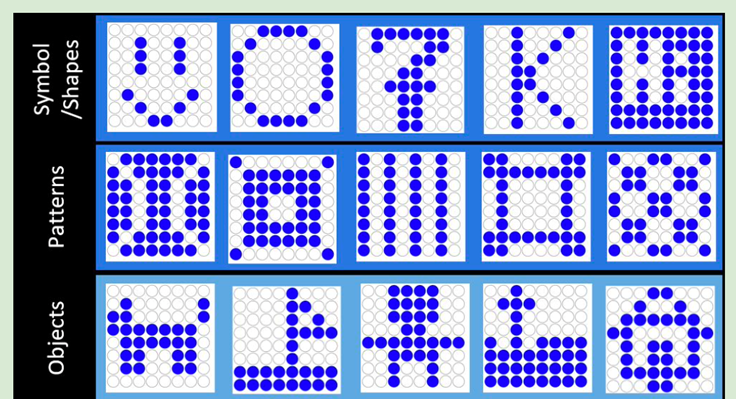
\includegraphics[width=0.7\textwidth]{images/diggs.png}
    \caption{Some creations from the free-play study on humans by \cite{diggs}. (Taken from the original publication.)}
    \label{fig:diggs}
\end{figure}
% \vspace{12pt}

\todo{Find more references on this bias towards semantics in cognitive science}
% Cedric Collas and Pierre-Yves Oudeyer have some papers on this bias towards semantics in developmental psychology.

In the context of artificial intelligence, self-supervised learning has been a topic of interest for researchers in the fields of robotics and machine learning (ML), and the ability to efficiently and sufficiently explore remains a fundamental challenge.
In recent years, reinforcement learning (RL) has emerged as a powerful framework for training agents to learn complex behaviors through trial and error.
However, most RL algorithms are designed to solve specific tasks and are not well-suited for free-form exploration.
Instead, complementary formulations of novelty-based or uncertainty-based exploration methods have been proposed to encourage agents to explore their environment in a self-supervised manner \citep{rnd,icm,disagreement,exploration_survey}. 
Yet, these methods are often unable to generate diverse and creative behaviors that are characteristic of human exploration.


\todo{Play vs exploration}

\todo{Comments on shaping of clip rewards near and far from the goal states}
% CLIP rewards are well-shaped around the goal state, whereas near the starting state, they are poorly shaped.

\todo{Comments on effects of model size from vlm rm}
% Finally, we investigate the effect of the scale of the pre-trained VLM on its quality as a reward
% model. We focus on the “kneeling” task and consider 4 different large CLIP models: the original
% CLIP RN50 (Radford et al., 2021), and the ViT-L-14, ViT-H-14, and ViT-bigG-14 from
% OpenCLIP (Cherti et al., 2023) trained on the LAION-5B dataset (Schuhmann et al., 2022).
% In Figure 4a we evaluate the EPIC distance to human labels of CLIP reward models for the four
% model scales and different values of α, and we evaluate the success rate of agents trained using the
% four models. The results clearly show that VLM model scale is a key factor in obtaining good reward
% models. We detect a clear positive trend between model scale, and the EPIC distance of the reward
% model from human labels. On the models we evaluate, we find the EPIC distance to human labels is
% close to log-linear in the size of the CLIP model (Figure 4b).
% This improvement in EPIC distance translates into an improvement in success rate. In particular,
% we observe a sharp phase transition between the ViT-H-14 and VIT-bigG-14 CLIP models:
% we can only learn the kneeling task successfully when using the VIT-bigG-14 model and obtain
% 0% success rate for all smaller models (Figure 4c). Notably, the reward model improves smoothly
% and predictably with model scale as measured by EPIC distance. However, predicting the exact
% point where the RL agent can successfully learn the task is difficult. This is a common pattern in
% evaluating large foundation models, as observed by Ganguli et al. (2022).

% image captioning

\todo{Better segregate the different exploration methods (maybe in methods)}

% - Vision Language Models
This thesis focuses on the role of visual semantic bias in shaping these choices, proposing that our innate visual preferences act as a compass, directing our attention and interactions during free play.
Our work tried to imbue artificial agents with a visual semantics bias, akin to that in humans.
We do this by leveraging large vision language models (VLMs).
Also termed "foundational models", these deep neural networks are trained on massive generic text and image datasets using the recent advances in self-supervised learning. 
The abstractions of natural language, which reflect the semantics of the world, allow them to learn efficient representations that essentially encapsulate human visual understanding.

% - VLM Applications
VLMs are capable of successfully transferring to a diverse range of downstream applications, such as visual detection, classification, and question-answering.
However, the use of foundation models for control and embodied intelligence is relatively new and under-explored.
% For example, pre-trained vision-language encoders,
% such as CLIP (Radford et al., 2021), have been used far beyond their original scope, e.g., for image
% generation (Ramesh et al., 2022; Patashnik et al., 2021; Nichol et al., 2021), robot control (Shridhar
% et al., 2022; Khandelwal et al., 2022), or story evaluation (Matiana et al., 2021).

% CLIPort (Shridhar et al., 2021) combines CLIP embedding with a transporter network to learn language-conditioned robot manipulation policies from demonstrations.
% The concurrent works of Khandelwal et al. (2021) and Parisi et al. (2022), study the use of CLIP and other self-supervised representation networks as a perception module for control tasks and observe they outperform traditional ImageNet-pretrained backbones.
% 
% In RL, pretraining has been used to improve the representations of the policy network. 
% Pretrained CLIP features have been used in various recent robotics papers to speed up control and navigation tasks.
% These features can condition the policy network [26] or can be fused throughout the visual encoder to integrate semantic information about the environment [37]. 
% The goal of these works is to improve the perception of the policy.
% Pretrained language models can also provide useful initializations for training policies to imitate offline trajectories [42, 27].
% These successes demonstrate that large pre-trained models contain prior knowledge that can be useful for RL. While the existing literature uses pre-trained embeddings directly in the agent, we instead allow the policy network to learn from scratch and only utilize pre-trained embeddings to guide exploration during training (Figure S2).
% We imagine that future work may benefit from combining both approaches.

% - VLM as Rewards
Recent work \citep{zest,negprompt,vlmrm,lamp} has shown that they can be used as effective abstractions to generate zero-shot rewards for language-guided goal-conditioned tasks.
There are also other studies on using VLMs for exploration \citep{vlmlang,vlmdistill} that use them for refining intrinsic reward signals by abstracting away pseudo-novelty. 

% - Entropy Rewards
Yet this is fundamentally different from our goal as we are specifically interested in creative semantic expression.
Moreover, the existing studies do not consider the free-form exploration paradigm that is of interest to us; they require a specific goal to be achieved, either self-generated or manually defined.
We instead use VLMs to generate exploratory intrinsic rewards that incentivize the agent to play with the environment and build something meaningful.
This reward is based on minimizing the entropy of a VLM's predictions over a set of creative possibilities that the environment offers.
Without any explicit goal specification, our controller exploits this reward to guide the agent to semantically expressive states, i.e. to automatically converge to a state that the VLM finds confidently meaningful.

\todo{Introduce the sparse nature of the rewards}

% - RaIR (Regularity as Intrinsic Reward)
Furthermore, since there is an implicit structure in meaningful creations, and given the compositional strategies for creative expression learned by humans during development \citep{symmetry,compositional} that favor symmetry and uniformity, we hypothesized that a complementary reward for this regularity \citep{rair} could promote semantic expression.

We tested our formulations in two rich creative environments: the puzzle Tangram and a pixel grid, where we were able to achieve the desired semantically expressive behavior in our planning agent.
% We show the effect of all the different bells and whistles in an ablation study.

This thesis provides a novel perspective on imbuing free-form creativity in artificial agents and furthers the use of VLMs as a source of rewards in robotics and AI.
